\phantomsection
\addcontentsline{toc}{chapter}{List of Figures}
\listoffigures
\clearpage

\phantomsection
\addcontentsline{toc}{chapter}{List of Tables}
\listoftables
\clearpage

\phantomsection
\addcontentsline{toc}{chapter}{Sources}
\chapter*{Sources}

\phantomsection
\printbibliography[heading=subbibintoc, nottype=online, nottype=software]

\phantomsection
\printbibliography[heading=subbibintoc, type=online, title=Websites]

\phantomsection
\printbibliography[heading=subbibintoc, type=software, title=Software]
\begin{comment}
Software-Name mit Versionsnummer und Link zur Website. Nur was für die konkrete Arbeit relevant ist. Das Sie die Arbeit mit Word geschrieben haben, ist irrelevant. Das sieht man. LaTeX auch.
\end{comment}
\clearpage

\phantomsection
\addcontentsline{toc}{chapter}{Abbreviations}
\chapter*{Abbreviations}
\begin{description}
    \item [\textbf{AI}] Artificial Intelligence
    \item [\textbf{AAII}] Affinity for AI Interaction
    \item [\textbf{AUROC}] Area Under the Receiver Operating Characteristics
    \item [\textbf{CNN}] Convolutional Neural Network
    \item [\textbf{DNN}] Deep Neural Network
    \item [\textbf{DVT}] Deep Vein Thrombosis
    \item [\textbf{ML}] Machine Learning
    \item [\textbf{XAI}] Explainable Artificial Intelligence
\end{description}
\clearpage

\phantomsection
\addcontentsline{toc}{chapter}{Glossary}
\chapter*{Glossary}
\begin{description}
    \item [\textbf{Artificial Intelligence}] Systems that display intelligent behaviour by analyzing their environment and taking actions – with some degree of autonomy – to achieve specific goals.
    \item [\textbf{Affinity for AI Interaction}] Tendency to actively engage in intensive AI interaction, as a key personal resource for coping with intelligent systems.
    \item [\textbf{Area Under the Receiver Operating Characteristics}] Important evaluation metric for checking any classification model’s performance.
    \item [\textbf{Black Box}] System which can be viewed in terms of its inputs and outputs (or transfer characteristics), without any knowledge of its internal workings.
    \item [\textbf{Convolutional Neural Network}] Convolutional neural networks are a class of artificial neural networks, most commonly used for processing structured arrays of data such as images..
    \item [\textbf{Deep Neural Network}] Deep neural networks are a powerful category of machine learning algorithms implemented by stacking layers of neural networks along the depth and width of smaller architectures.
    \item [\textbf{Deep Vein Thrombosis}] Deep vein thrombosis occurs when a blood clot forms in one or more of the deep veins in your body, usually in the legs.
    \item [\textbf{Explainable Artificial Intelligence}] Artificial intelligence in which the results of the solution can be understood by humans.
    \item [\textbf{Machine Learning}] Machine learning is a branch of artificial intelligence (AI) and computer science which focuses on the use of data and algorithms to imitate the way that humans learn, gradually improving its accuracy.
\end{description}
\clearpage

\phantomsection
\addcontentsline{toc}{chapter}{Appendices}
\chapter*{Appendices}
\begin{comment}
Zusätzliche Informationen die zu lang für die Arbeit sind können hier verfügbar gemacht werden.

Aber auch an die DVD denken — was ist dort besser aufgehoben? Die Zeiten, in denen man Programmcode manuell eingetippt hat, sind ja glücklicherweise lange vorbei, deswegen macht Code hier wenig Sinn.

Ist entsprechend ein Priorisierung: Was würde sich der Leser vielleicht gerne während des Lesens der Arbeit (z. B. im Zug) ansehen, wenn er auch gerade nicht auf die DVD zugreifen kann (kein DVD Laufwerk)?

Inhalte sind oft: Überblick der Inhalte der DVD, Fragebögen (falls digital Screenshots oder neu für den Druck formatiert), Interviewleitfäden, etc. Selten detailliertere Evaluationsergebnisse.

Hier kurz die Zwischenüberschriften nennen und evtl. 1 Satz, was dort zu finden ist (falls es nicht schon durch die Zwischenüberschrift klar ist). 
\end{comment}

Text \dots

\phantomsection
\addcontentsline{toc}{section}{Appendix A: Inhalt der DVD}
\section*{Appendix A: Inhalt der DVD}
\begin{comment}
Oft ein Default: Was findet man auf der beiliegenden DVD in welchem Verzeichnis? Max. 1 Seite.

\textbf{In jedem Fall} die PDF der Arbeit, den Programmcode, Daten (anonymisiert!).

\textbf{Niemals} Interviewaufzeichnungen, Einverständniserklärungen oder ähnliche personenbezogene Daten auf die DVD brennen — Sie haben in den meisten Fällen Anonymität zugesichert und die DVD ist frei zugänglich (ein Exemplar der Arbeit kommt in die Bibliothek). 
\end{comment}

Text \dots

\phantomsection
\addcontentsline{toc}{section}{Appendix B: Interview Guideline}
\section*{Appendix B: Interview Guideline}\label{appendix:interview_guideline}
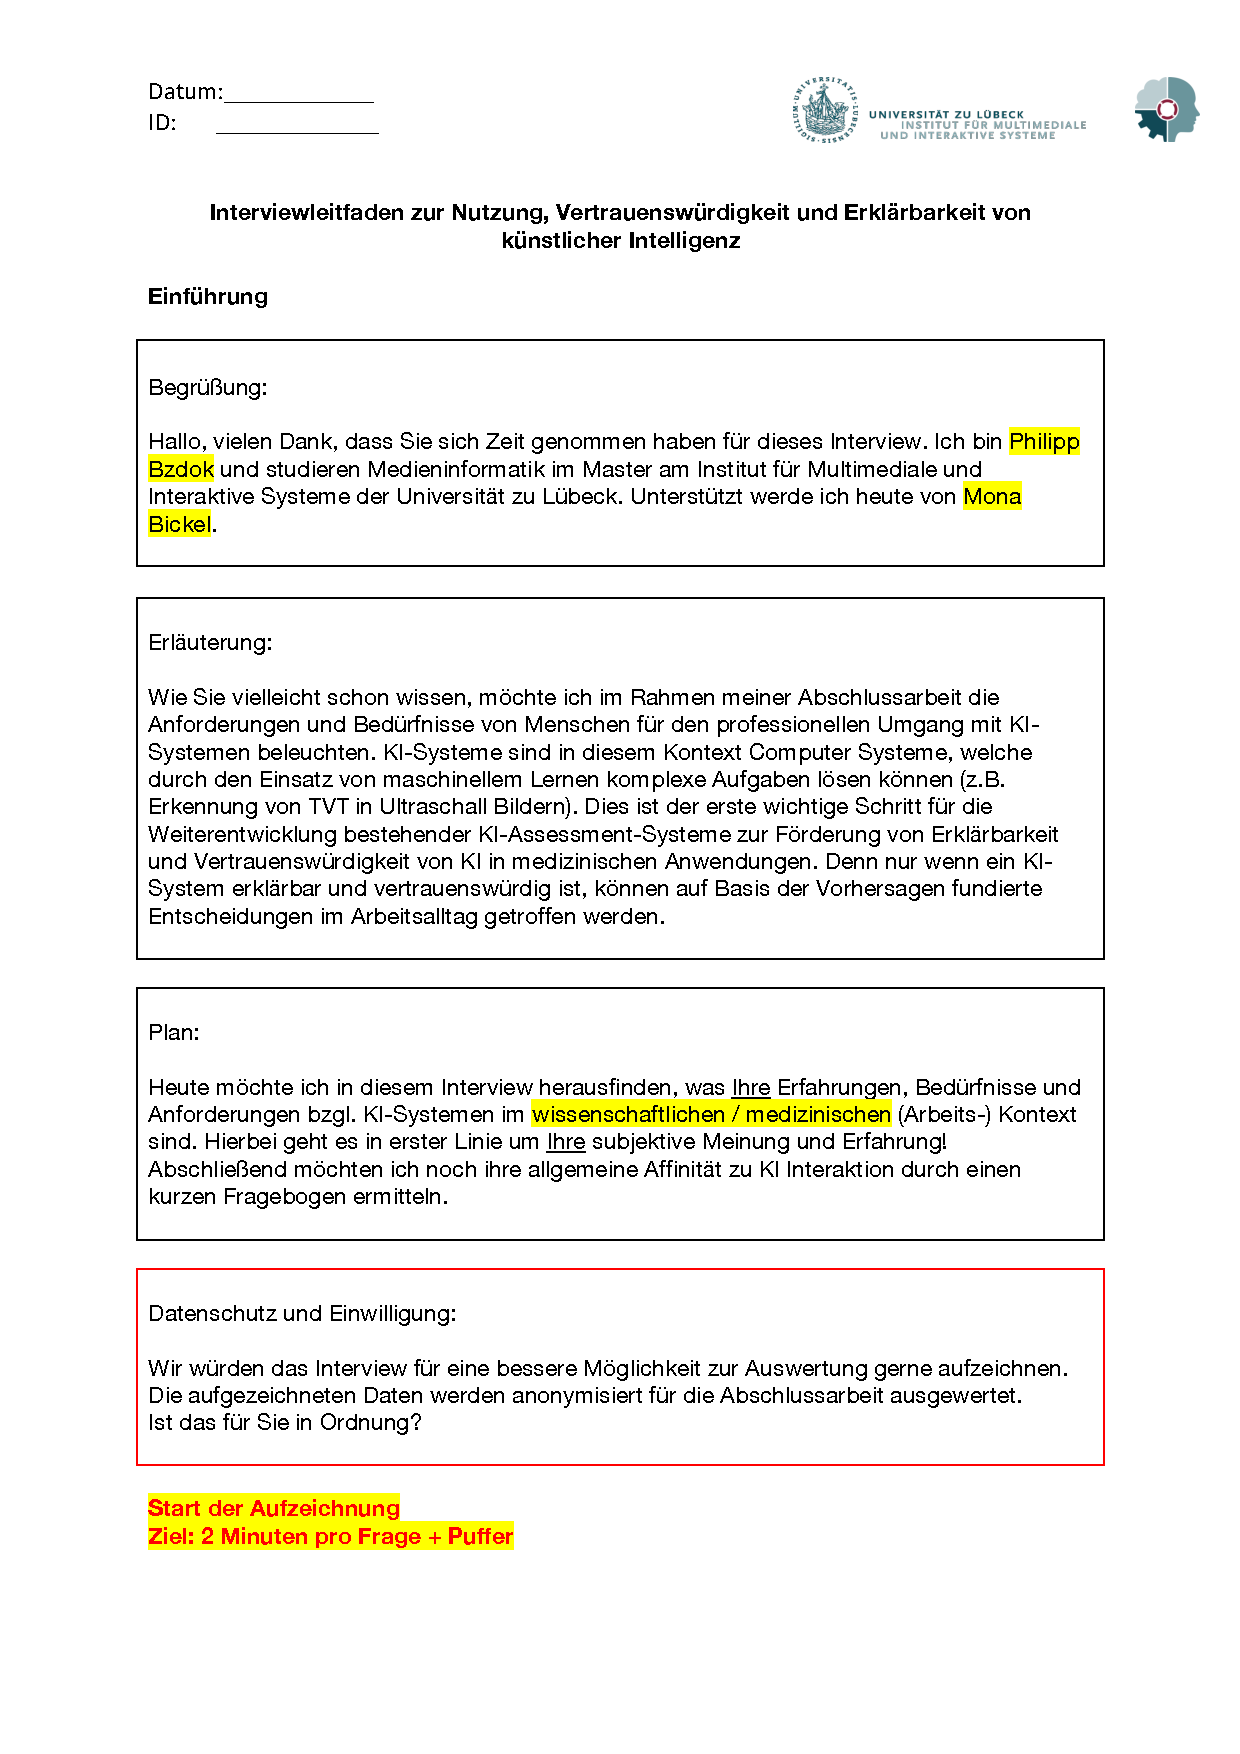
\includepdf[pages=-]{docs/Interviewleitfaden_v4.pdf}

\clearpage

\phantomsection
\addcontentsline{toc}{chapter}{Assertion under Oath}
\chapter*{Assertion under Oath}
I declare in lieu of an oath that I have written this paper independently and have used only the sources indicated.

\begin{comment}
[Nach Ausdruck unterschreiben. Muss auf Papier sein.]
\end{comment}

-----------------------------------------------------------------

Lübeck, \today, \authorMA